% Muster für die Seminarausarbeitung
% HPI Potsdam

\documentclass[11pt, a4paper]{article}

\usepackage{ngerman}
\usepackage[utf8]{inputenc} %Korrekte Kodierung der Umlaute nach UTF-8
\usepackage[T1]{fontenc} %Korrekte Kodierung der Umlaute nach UTF-8
\usepackage{amsfonts}
\usepackage{amssymb}
\usepackage{epsfig}   % Zum Einbinden von Bildern
\usepackage{url}      % Korrekter Satz von URLs
\usepackage{soulutf8}
\usepackage{color}    % Verwendung von Farben
\usepackage{listings} % Korrekter Satz von Listings und Quellcode


%Hilfs-Fonts - ohne Serifen (hier für Tabellen)
\newfont{\bib}{cmss8 scaled 1040}
\newfont{\bibf}{cmssbx8 scaled 1040}

\definecolor{lightgray}{gray}{0.85}

%Seitenformat-Definitionen
\topmargin0mm
\textwidth147mm
\textheight214mm
\evensidemargin5mm
\oddsidemargin5mm
\footskip19mm
\parindent=0in

\begin{document}          

\begin{titlepage}
  \begin{center} 
    \mbox{}
    \vspace{1cm}
    
    {\huge Titel der Seminararbeit \\[1em] {\LARGE ggf.~mit Untertitel}}  
        
    \vspace{5cm}
    
    Seminararbeit im Seminar \\[1em]
    {\large \sc Titel des Seminars} \\[1em]
    Sommersemester 20XX \\[1em]
    Hasso-Plattner-Institut für Softwaresystemtechnik GmbH \\[1em]
    Universität Potsdam
    
    \vspace{4cm}
    
		vorgelegt von
		
    \vspace{1em}
    
		{\Large Maximilian Mustermann} \\
		{\Large Alfred E. Neumann}
		
    \vspace{4em}
    
    18.~April 20XX
  \end{center}
\end{titlepage}


\setcounter{page}{1}

% Zweite Seite = Kurzzusammenfassung
\begin{center}
{\bf Kurzzusammenfassung} 
\end{center}

\noindent
An dieser Stelle erfolgt eine knappe Zusammenfassung der vorliegenden Arbeit ([engl.] Abstract)\index{Abstract}, die maximal ca.~200 Worte umfassen sollte. 
Der Sinn und Zweck dieser Kurzzusammenfassung liegt darin, einem interessierten Leser die Entscheidung zu erleichtern, die vorliegende Arbeit überhaupt zu lesen bzw.~vor dem Lesen der Arbeit erst einmal in Erfahrung zu bringen, worum es geht.
Also eine knappe, motivierende Hinführung zum Problem und wie sie es gelöst haben.

\bigskip

Wenn Sie eine Kurzzusammenfassung schreiben, bedenken Sie, dass diese oft auch alleine publiziert wird, d.h. sie sollte unabhängig vom nachfolgend explizit dargestellten Inhalt der Arbeit für den Leser verständlich sein.
Daher ist es immer sinnvoll, diese Zusammenfassung erst ganz am Ende zu schreiben, wenn Sie die eigentliche Arbeit bereits abgeschlossen haben.

\newpage

% Dritte Seite = Inhaltsverzeichnis
\tableofcontents 

\newpage

% Vierte Seite = Hier geht's eigentlich richtig los
\section{Einleitung}
\label{sec_einleitung}

\noindent
Mit den vorliegenden Hinweisen versuchen wir Ihnen einen Leitfaden zum Erstellen von Seminararbeiten im Fach Informatik an die Hand zu geben.
Wie Sie sicher schon beim Lesen wissenschaftlicher Arbeiten bemerkt haben werden, folgen diese meist einem einheitlichen Aufbau.
Dies liegt nicht daran, dass die Autoren sich keine Mühe geben würden bzw. große Langweiler sind, denen eben nichts Neues einfallen würde.
Nein, ein einheitlicher Aufbau erleichtert dem Leser -- der meist nie besonders viel Zeit hat bzw. investieren möchte -- die wesentlichen Beiträge der Arbeit schnell und effizient zu erfassen.


\subsection{Die Gliederung}
Aber wie gliedert man eine wissenschaftliche Arbeit?
Meist kommt dabei das folgende einfache Schema zum Einsatz:\index{Aufbau der Arbeit}
\begin{enumerate}
\item Einleitung
\item Verwandte Arbeiten und wissenschaftlicher Hintergrund (Related Work)
\item Eigener Ansatz zur Lösung der gestellten Aufgabe -- dies können gerne mehrere Kapitel werden...
\item Diskussion der erzielten Ergebnisse
\item Zusammenfassung und Ausblick 
\end{enumerate}

Auf die Eigenheiten der einzelnen Unterpunkte werden wir im Folgenden noch genauer eingehen.
Beginnen wir einfach mit der Einleitung.\index{Einleitung}

\subsection{Inhalt der Einleitung}
Die Einleitung soll den Leser zum {\bf Thema\index{Thema} hinführen}, die Arbeit in einen Gesamtzusammenhang einordnen und einen kurzen Überblick über den Inhalt der Arbeit geben. 
Dabei sind die folgenden Punkte besonders wichtig:

\begin{itemize}
\item Motivation\index{Motivation} des Themas -- warum ist das Thema überhaupt von Bedeutung?
\item Wie ordnet sich das Thema in einen größeren Gesamtzusammenhang (z.B. den Rahmen des Seminars) ein?
\item Darlegung der grundlegenden Aufgabe: Worum geht es eigentlich? Was sind die zentralen Fragestellungen? Wie beabsichtigen wir diese zu lösen?
\item Warum lohnt sich das Weiterlesen? 
\end{itemize}
Wichtig ist, dass die Einleitung die {\bf Dramaturgie} der Arbeit quasi wie einen \glqq roten Faden\grqq\, sichtbar werden lässt.

\bigskip

Am Ende der Einleitung sollte ein \textbf{kurzer Überblick über den Inhalt} der einzelnen Kapitel folgen. 
Die vorliegende Arbeit könnte wie folgt skizziert werden:

\bigskip

Kapitel~\ref{sec_aufbau} gibt Hinweise zum Aufbau einer Seminararbeit und wie deren Inhalte zu gestalten sind.
Kapitel~\ref{sec_stil} gibt allgemeine Hinweise zur Formatierung von wissenschaftlichen Arbeiten.
In Kapitel~\ref{sec_inhalt} werden die einzelnen inhaltlichen Bestandteile der wissenschaftlichen Arbeit dargestellt, worauf in Kapitel~\ref{sec_literatur} wichtige Hinweise zur korrekten Zitierweise gegeben werden.
Kapitel~\ref{sec_conclusion} beschließt die Arbeit mit einer Zusammenfassung der Ergebnisse und einem Ausblick auf die weitere Entwicklung des eigentlichen Themas.


 
\newpage
%
\section{Aufbau und Inhalt der Seminararbeit}
\label{sec_aufbau}

Im vorangegangenen Kapitel hatten wir bereits die Gliederung einer Seminararbeit kurz vorgestellt und erläutert, welche inhaltlichen Punkte in der \glqq Einleitung\grqq\, behandelt werden sollten.
Die folgenden Abschnitte skizzieren inhaltlich die übrigen der bereits genannten Gliederungspunkte.

\subsection{Verwandte Arbeiten und wissenschaftlicher Hintergrund (Related Work)}
%%
Hier sind vor allem zwei inhaltliche Punkte zu berücksichtigen:
\begin{itemize}
\item {\bf Notwendige Vorarbeiten und Grundlagen, die zum Verständnis der Arbeit notwendig sind}

Keine bzw. kaum eine Arbeit beginnt als \glqq tabula rasa\grqq , d.h. meist bauen wir auf  vorhandenen Grundlagen bzw. Vorarbeiten auf.
Die zum Verständnis der eigenen Arbeit notwendigen Grundlagen und Voraussetzungen müssen in diesem Kapitel skizziert bzw. zusammengefasst werden.
Dabei sollte man vom durchschnittlichen Kenntnisstand eines Informatikers ausgehen, d.h. Allgemeinplätze und allzu Grundlegendes hat hier nichts zu suchen.
Genauso soll hier nicht notwendigerweise eine kompletter Wissenschaftszweig in epischer Tiefe ausgebreitet werden, sondern lediglich die zum Verständnis notwendigen Teilbereiche in skizzenhafter Form und mit Angabe von Literaturhinweisen zusammengefasst werden. (Zum Beispiel können hier die Grundlagen und Vorzüge von Linked Open Data erläutert werden.)

\smallskip

\item {\bf Alternative Ansätze und ggfs. Forschungsarbeiten zum Thema}
Besonders wichtig ist es, spezielle Vorarbeiten und alternative Ansätze zum behandelten Thema darzulegen.
Gibt es zu der von Ihnen gewählten Problemstellung alternative Lösungen, die einen anderen oder vergleichbaren Ansatz verfolgen? Wie unterscheiden sich diese Lösungen von Ihrem Vorschlag, wo liegen Vor- und Nachteile des jeweiligen Ansatzes?

Wichtig ist, dass Sie jede der vorgestellten Arbeiten 
\begin{itemize}
\item korrekt zitieren (Bibliografie),
\item kurz die wichtigsten Ergebnisse bzw. Strategien skizzieren und
\item diese (kurz und knapp) in Zusammenhang mit ihrer eigenen Arbeit stellen. 
\end{itemize}
Wie unterscheidet sich der eigene Ansatz von den vorgestellten Arbeiten? 
Warum ist der eigene Ansatz eventuell erfolgsversprechender? 

\end{itemize}

\subsection{Eigener Ansatz zur Lösung der gestellten Aufgabe}
%%
Hier haben Sie die Freiheit, Ihren eigenen Arbeiten angemessen viel Raum zur Verfügung zu stellen.
Achten Sie dabei auf einen logischen Aufbau der Darstellung, d.h. Grundlegendes zuerst.
\begin{itemize}
\item Wie sind Sie vorgegangen?
\item Wo gibt es Probleme?
\item Wie werden diese gelöst?
\item Schreiben Sie in verständlicher Weise und drücken Sie sich dabei jeweils möglichst präzise, d.h. unmissverständlich aus (vgl. Kap.~\ref{sec_stil})
\item Verwenden Sie Abbildungen, Tabellen und Beispiele.
\item Setzen Sie kein Wissen als implizit vorhanden voraus, sondern sprechen Sie explizit alle Probleme und wichtigen Fakten an.
\item Wichtig: Was Sie hier nicht beschreiben, können wir nicht bewerten!
\end{itemize}
Bedenken Sie dabei stets, dass ein Leser nicht dasselbe Wissen besitzen kann wie Sie und das Sie ihm deshalb ihre Ergebnisse erklären müssen.


\subsection{Diskussion der erzielten Ergebnisse}
%%
In diesem Kapitel sollten Sie Ihre Ergebnisse präsentieren.
Dabei sollten (falls jeweils zutreffend) folgende Fragen beantwortet werden:
\begin{itemize}
\item Was wurde erreicht, was kann noch verbessert werden bzw. wo gibt es noch offene (evtl. aus Zeitgründen nicht implementierte) Punkte?
\item Warum ist der eigene Ansatz besser/schlechter als die zum Vergleich herangezogenen?
\item Was haben Sie aus dem Seminar mitgenommen (z.B. Wo liegen die Vorteile von Linked Open Data?)
\end{itemize}


\subsection{Zusammenfassung und Ausblick}

In diesem Abschnitt sollten die erzielten Ergebnisse noch einmal kurz zusammengefasst werden und ein Ausblick auf weiterführende Entwicklungsarbeiten gegeben werden (vgl. Kap.~\ref{sec_conclusion}). Hier können Sie z.B. ausführen, welche Arbeiten Sie aus Zeitgründen nicht umsetzen konnten, aber für wichtig oder sinnvoll erachten.
\newpage
%
\section{Nützliches und Wissenswertes zum Erstellen einer Seminarausarbeitung}
\label{sec_stil}

\subsection{Allgemeine Hinweise}
Ganz allgemein handelt es sich bei der Seminarausarbeitung bereits um eine {\bf wissenschaftliche Arbeit}.
Begehen Sie nicht den Fehler und sehen Sie diese als wortwörtliche Wiedergabe Ihres Seminarvortrags an, sondern beachten Sie stets die folgenden Punkte:
\begin{itemize}
\item Die sprachliche Darstellung sollte dem Rahmen angepasst sein und stets auf einer sachlichen Argumentationsebene rangieren.
\item Der Schreibstil sollte unpersönlich gehalten werden. 
Vermeiden Sie Sätze, die die Wörter "`wir"', "`uns"', "`Sie"' usw.~enthalten.\footnote{Eine Ausnahme von dieser Regel stellen persönliche Kommentare, Bewertungen oder Urteile von Sachverhalten dar. Hier sollte klar werden, dass es sich um Ihre eigene Leistung handelt.}
\item Vermeiden Sie (Bandwurm-)Sätze, die sich über mehr als 2--3 Zeilen ziehen. Sie erhöhen damit signifikant die Lesbarkeit Ihrer Arbeit.
\item Vermeiden Sie sprachliche Komplexität, d.h. beschränken Sie die Anzahl der notwendigen Nebensätze auf ein Mindestmaß.
\item Drücken Sie sich einfach und präzise aus. Vermeiden Sie eine \glqq geschraubte\grqq\, Ausdrucksweise.
\item Achten Sie auf temporale Konsistenz in der Verwendung von Präsens oder Präteritum  bei Verben.
\item Vermeiden Sie Worthülsen und unnötige Redewendungen ohne signifikanten Inhalt. 
\item Legen Sie Ihren Standpunkt stets mit der angemessenen Objektivität dar, auch wenn es um die Bewertung von Vor- oder Nachteilen des jeweiligen Themengegenstandes geht.
\item Vermeiden Sie unnötige Anglizismen (z.B.~"`connecten, downloaden, backupen"').
Existiert in diesem Zusammenhang bereits eine deutsche Redewendung, dann benutzen Sie diese (z.B. "`öffentlicher Schlüssel"' statt "`public key"').
Verwenden Sie englische Begriffe, so passen Sie diese entsprechend den deutschen Rechtschreibregeln bez.~Flexion, Silbentrennung, Getrennt- und Zusammenschreibung an.
\item Wenn Sie Begriffe einführen bzw. verwenden, deren Bedeutung nicht unmittelbar auch einem Nichtfachmann geläufig ist, sollten diese stets erläutert werden. 
Die Fachbegriffe sollten unmittelbar im Text erklärt werden. 
In natur- und. ingenieurwissenschaftlichen Arbeiten ist es eher unüblich, Erklärungen in Fußnoten zu platzieren. 
\item Achten Sie auf einen {\bf logischen Aufbau} Ihrer Arbeit, sowie ihrer einzelnen Unterkapitel und Gliederungspunkte.
\item {\bf Dringende Empfehlung:} Lassen Sie Ihre Ausarbeitung am besten von einem "`Nichtfachmann"'/einer "`Nichtfachfrau"', also nicht von einem Informatiker/einer Informatikerin Korrekturlesen.
Auf diese Weise werden Schwachstellen in Ihrer Argumentation und andere logische Mängel am deutlichsten.
\item Verwenden Sie konsequent die {\bf neue deutsche Rechtschreibung}.
Lassen Sie Ihren Text von einem Rechtschreibprogramm prüfen.
Allerdings kann dieses nur die korrekte Schreibweise von Einzelwörtern und nicht die korrekte Verwendung von Einzelwörtern im Satzzusammenhang überprüfen, insbesondere wenn es um grammatikalische Fehler oder Kommasetzung geht.
Verlassen Sie sich daher nicht alleine auf das Programm.
\item In deutschen Texten werden anstelle der englischen ''Quotes'' die Anführungsstriche in Form von "`Gänsefüßchen"' geschrieben. 
In dem Textsatzsystem {\LaTeX} stehen hierfür z.B. die Befehle \verb|\glqq| und \verb|\grqq| zur Verfügung. \\
{\bf Achtung:} Dazu muss das Paket {\tt ngerman} in den Header eingebunden werden.
\end{itemize}



\subsection{Weitere Formatierungshinweise}
\subsubsection{Abbildungen}
Abbildungen sind für das Erläutern und Verdeutlichen von komplexen Strukturen und Abläufen, wie sie üblicherweise in wissenschaftlichen Arbeiten beschrieben werden, unverzichtbar.
Die Abbildungen in Ihrer Arbeit sind stets zu {\bf nummerieren} und wie folgt zu setzen (siehe Abb.~\ref{fig_Abb1}).
%Hier eine Abbildung
\begin{figure}[ht]
  \begin{center}
  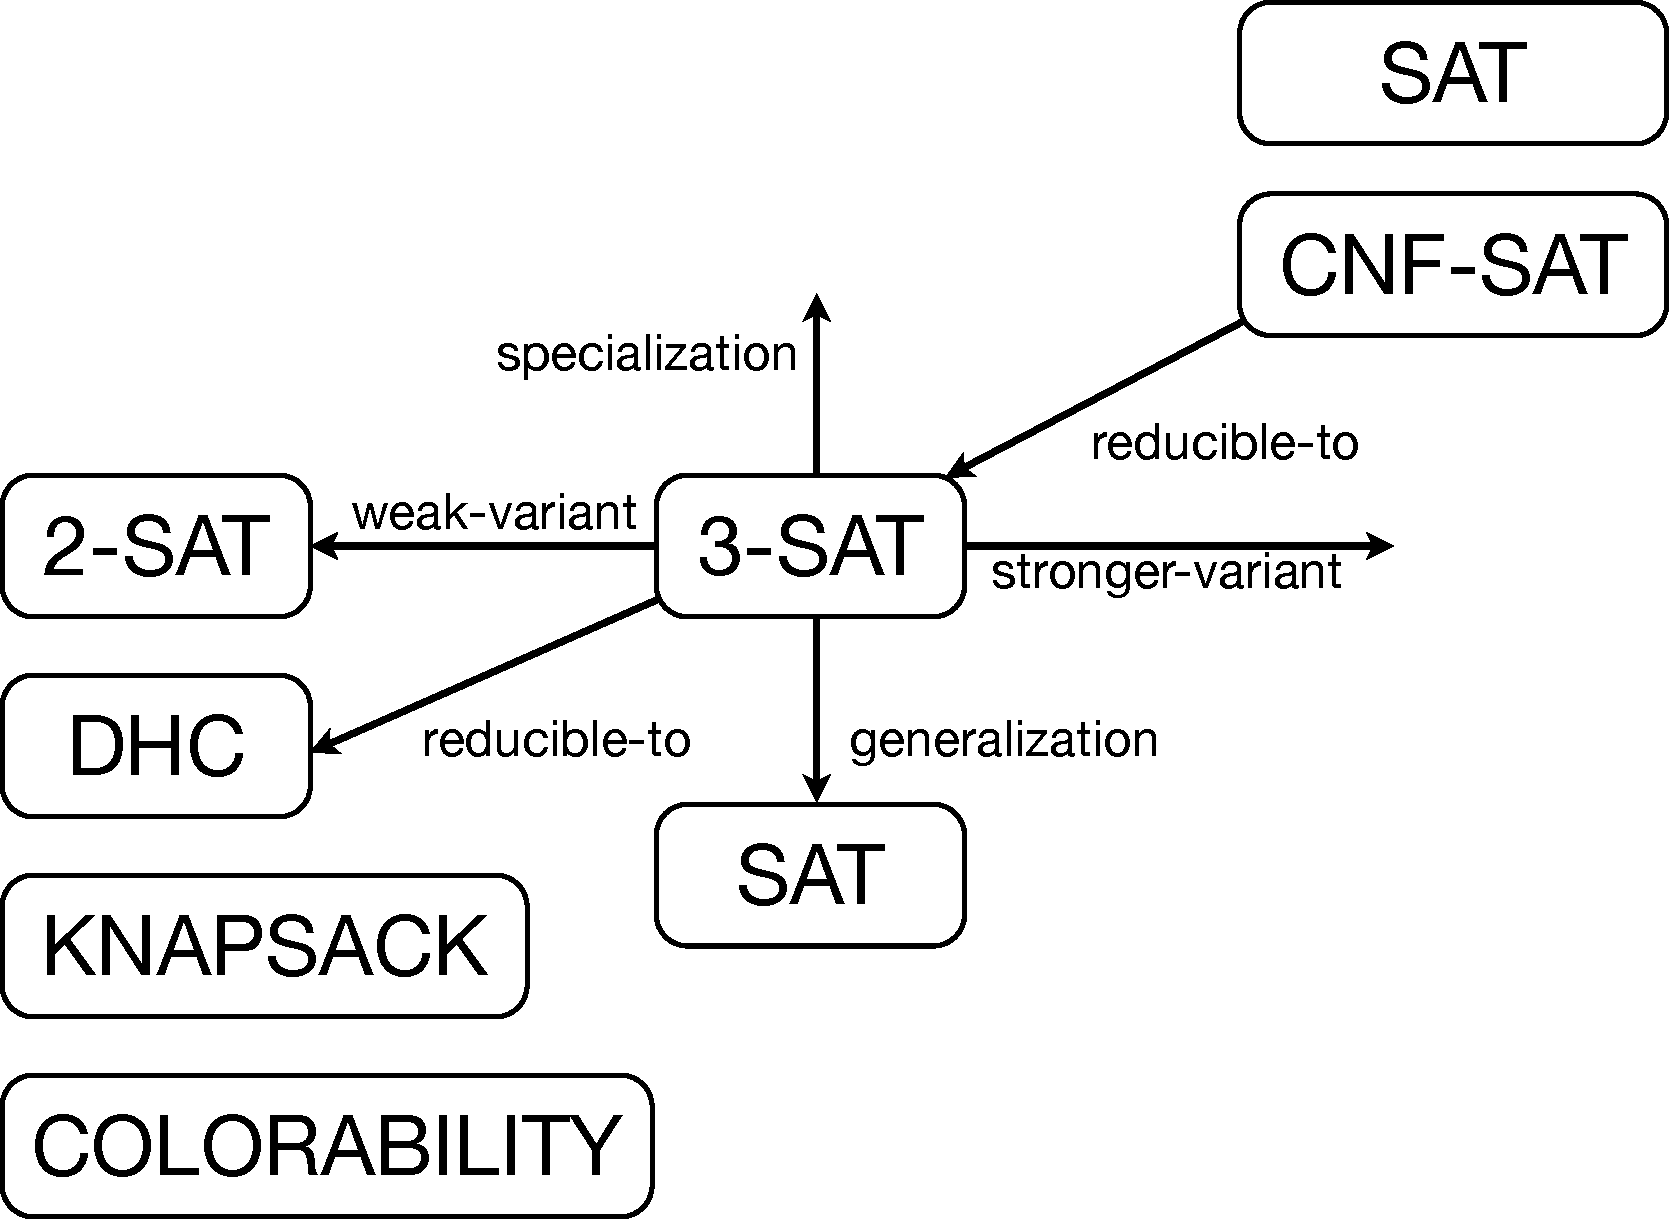
\includegraphics[width=0.5\textwidth]{images/3sat.pdf}
  \end{center}
  \caption{Das Umfeld des 3-SAT Problems}
  \label{fig_Abb1}
\end{figure} 

Jede Abbildung soll neben einer Abbildungsnummer eine Bildunterschrift ("`Das Umfeld des 3-SAT Problems"') besitzen, die die Grafik näher erläutert.
Weiterhin ist darauf zu achten, dass zu jeder Abbildung eine Bezugnahme im Text aufgenommen wird, d.h. an geeigneter Stelle sollte ein Verweis der Form (siehe Abb.~\dots) erfolgen.

Beachten Sie bitte, dass es sich bei der vorliegenden Grafik um eine .eps-Datei handelt (Encapsulated Postscript), die mit Hilfe des \LaTeX-Pakets {\tt epsfig} eingebunden wurde.
Die Abbildung kann natürlich auch mit Hilfe anderer Pakete eingebunden werden.
Achten Sie dabei aber stets auf eine für den Druck geeignete Bildqualität!

\smallskip

\begin{center}
\colorbox{lightgray}{
\parbox{140mm}{
{\bf Achtung:} \\
Eine Abbildung sollte nicht einfach per "`copy and paste"' aus dem WWW in Ihre Ausarbeitung übernommen werden. 
Einerseits leidet im Allgemeinen bei einer solchen Vorgehensweise die Qualität bei einer entsprechenden Vergrößerung für die Druckaufbereitung stark darunter (siehe Abb.~\ref{fig_Abb2}), anderseits muss sichergestellt werden, dass der Urheber der Originalgrafik damit einverstanden ist, dass die Grafik in die Seminararbeit aufgenommen wird.
Der sicherste Weg ist deshalb, die Grafik mit einem geeigneten Grafikprogramm {\em selbst} zu erzeugen und anschließend in den Text einzubinden.}}
\end{center}

%Hier eine Abbildung
\begin{figure}[ht]
  \begin{center}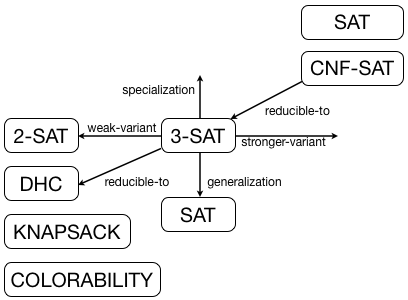
\includegraphics[width=0.5\textwidth]{images/3sat.png}\end{center}
  \caption{So sollte eine Abbildung nicht aussehen (JPG-Grafik, "`copy and paste"')}
  \label{fig_Abb2}
\end{figure} 
Verwenden Sie eine Abbildung, die in dieser Form bzw. in einer sehr ähnlichen Form bereits veröffentlicht wurde, müssen Sie dies durch eine bibliografische Referenz deutlich machen, d.h. Sie müssen wie bei einem Zitat die Fundstelle im Text als Literaturangabe aufnehmen.



\subsubsection{Tabellen}
Für Tabellen gilt dasselbe wie für Abbildungen.
Setzen Sie Tabellen nie in den Fließtext, sondern in die entsprechende \LaTeX-Tabellenumgebung und versehen Sie diese ebenfalls mit einer {\em Tabellennummer} und einer Tabellen{\em überschrift} (siehe Tabelle \ref{tab_HistoryWWW}).

%Hier eine Tabelle
\begin{table}
\caption{Die Geschichte des World Wide Web}
\begin{tabular}{rp{12cm}} \noalign{\smallskip} \hline \noalign{\smallskip}
{\bf 1945} & Vennevar Bush beschreibt MEMEX: das erste Hypertextsystem.\\
{\bf 1965} & Ted Nelson prägt als erster das Wort {\bf Hypertext} auf der ACM-Jahreskonferenz.\\ 
{\bf 1968} & Doug Engelbart entwickelt ein Hypertext-basiertes Prototypensystem NLS und erfindet zu diesem Zweck die Maus als Eingabegerät.\\
{\bf 1980} & Tim Berners Lee schreibt ein erste Notizbuch-Programm mit Hypertextlinks.\\
{\bf 1989} & Tim Berners Lee verfasst ein erstes Memorandum zu seinem Hypertext-Dokumentenverwaltungssystem am Kernforschungszentrum CERN.\\
{\bf 1990} & Zusammen mit Robert Cailliau entwickelt Tim Berners Lee den ersten WWW-Server und WWW-Browser: die Geburtsstunde des WorldWideWeb.\\  \noalign{\smallskip} \hline
\end{tabular}
\label{tab_HistoryWWW}
\end{table}  

\noindent
Grundsätzlich sollte man bei dem Setzen einer Tabelle sparsam mit grafischen Elementen -- wie Hilfslinien oder bunte Tabellenunterlegungen -- umgehen, da diese die Lesbarkeit sehr stark beeinträchtigen können.


\subsubsection{Listings, Quellcode und Pseudocode}

Sollten Sie Quellcode eines Programmes mit in Ihre Arbeit aufnehmen oder einen Algorithmus mit Hilfe von Pseudocode veranschaulichen, sind diese im Sinne einer Abbildung (siehe Abb.~\ref{fig_Abb3}) zu behandeln.
Ebenso wie eine Abbildung sind Listings, Quellcode oder Pseudocode jeweils mit einer laufenden Nummer und einer Bildunterschrift zu versehen.

\begin{figure}[ht]
\lstset{language=c++}
\lstset{backgroundcolor=\color{lightgray}}
\begin{lstlisting}{}
    for( i = 0; i < 10; i++ )
    {
        for( j = 0; j < 10; j++ )
        {
            // calculate $a_{ij}$
            a[i][j] = b[j][i];
        }
    }

\end{lstlisting}
  \caption{Einbinden von Quellcode in die Arbeit}
  \label{fig_Abb3}
\end{figure}

Sie können Listings z.B. mit Hilfe des \LaTeX-Pakets {\tt listings} einbinden.
Insbesondere, wenn längere Quellcode-Passagen in den Text eingebunden werden sollen, empfiehlt sich diese Vorgehensweise, da das Paket automatisch Seitenumbrüche korrekt formatiert und auch die Verwendung von internen Zeilennummern ermöglicht.

\subsubsection{Mathematische Formeln}

{\LaTeX} bietet sich insbesondere als Textverarbeitungssystem an, wenn es um das korrekte Formatieren mathematischer Ausdrücke und Formeln geht.
Versehen Sie alle Formeln, die Sie in Ihrer Arbeit verwenden -- insbesondere diejenigen, auf die Sie später noch Bezug nehmen --  mit einer entsprechenden Nummerierung.

\begin{equation}\label{formel1}
\frac{\sum_{n > 0} z^n}
{\prod_{1\leq k\leq n} (1-q^k)}
\end{equation}


\subsubsection{{\LaTeX} und andere Textverarbeitungssysteme}
Wenn Sie das Textsatzsystem {\LaTeX} für die Erstellung der Ausarbeitung verwenden, dann benutzen Sie das vorliegende \LaTeX-Musterdokument als Layoutvorlage für Ihre Arbeit.
Sollten Sie ein anderes Textverarbeitungsprogramm als {\LaTeX} verwenden, dann halten Sie sich bitte an die in diesem Beispieldokument verwendeten Bemaßungen und Formatierungen.
Sie können sich z.B.~dieses Beispieldokument ausdrucken und die entsprechenden Maßangaben, wie 
\begin{itemize}
\item linker, rechter Rand
\item Abstand oben, unten
\item etc.
\end{itemize}
abmessen und in Ihrem eigenen Textverarbeitungsprogramm verwenden. \\
Denken Sie bitte daran, dass neben einer gedruckten Version Ihrer Seminarausarbeitung auch eine {\bf pdf}-Datei abzugeben ist.
Diese können Sie zusammen mit Ihrer Präsentation (pdf-Datei + evtl.~ppt-Datei) via E-Mail zusenden.

\newpage
%
\section{Inhaltliche Bestandteile der Seminararbeit}
\label{sec_inhalt}

\subsection{Gliederungspunkte}

Die Seminarausarbeitung sollte {\bf ohne} die Standardseiten wie
\begin{itemize}
\item Titelseite
\item Kurzzusammenfassung
\item Inhaltsverzeichnis
\item Literaturverzeichnis
\end{itemize}
tatsächlich {\bf 15 Seiten} umfassen!

\subsection{Inhalt der Gliederungspunkte}
Unterteilen Sie den eigentlichen Text Ihrer Arbeit in logische, inhaltlich aufeinander aufbauende Gliederungspunkte.
Stellen Sie sicher, dass der Inhalt jedes Gliederungspunktes auch mit dessen einleitenden Sätzen übereinstimmt.
Achten Sie bei der Erstellung der einzelnen Gliederungspunkte auf den sprichwörtlichen "`roten Faden"' , der sich durch die Arbeit ziehen sollte.
Reihen Sie nicht nur einzelne Fakten hintereinander, sondern bringen Sie diese in einen logischen Zusammenhang.
Dies gilt auf allen Gliederungsebenen, d.h.~sowohl für den Gesamtaufbau der Arbeit wie auch für die einzelnen Unterkapitel.

Hüten Sie sich vor Plagiaten!
Dem Vorwurf des Plagiats setzt man sich auch dann aus, wenn man einer anderen Arbeit zu dicht folgt und seine eigene Arbeit zu sehr an eine andere Arbeit anlehnt.
Die Suchmaschine Google und das WWW bieten einen reichen Schatz an studentischen Arbeiten zu den verschiedensten Themen.
Aber bedenken Sie:
\begin{itemize}
\item Ihr Dozent ist ebenfalls in der Lage, einen Browser zu bedienen.
\item Was Sie im WWW finden, kann auch Ihr Dozent finden.
\item Ihr Dozent hat in der Regel einen besseren Überblick über bereits bestehende Arbeiten zum Thema als Sie.
\item Ihr Dozent hat bereits vor Ihnen eine WWW-Recherche zum Thema durchgeführt.
\end{itemize}
Grundsätzlich können Sie fremde Quellen immer zu Rate ziehen und diese korrekt zitieren.
Eine komplette Arbeit einfach abzuschreiben bringt allerdings auch Ihnen persönlich weder einen Erkenntnisgewinn noch Erfahrungen im Erstellen einer wissenschaftlichen Arbeit.


\subsection{Umfang der Gliederungspunkte}
Die einzelnen Unterkapitel sollten entweder selbsterklärend sein bzw.~sollte sich deren Zusammenhang aus den bereits vorangegangenen Kapiteln erschließen.
Ist dies nicht der Fall, müssen Sie eventuell die einzelnen Kapitel umorganisieren bzw. zusätzliche Erklärungen einfügen.

\subsection{Logischer Zusammenhang}
Generell gilt auch hier: Lesen Sie Ihre Arbeit am Ende komplett in einem Stück durch.
Wenn Sie glauben, Ihre Arbeit sei logisch konsistent und vollständig, dann lassen Sie diese von einer unbeteiligten Person (am besten einem Nichtfachmann/einer Nichtfachfrau) noch einmal durchlesen.
Diese wird Sie auf eventuell bestehende logische Unzulänglichkeiten hinweisen.

\newpage
%
\section{Das Literaturverzeichnis und die korrekte Zitierweise}
\label{sec_literatur}

\subsection{Was wird zitiert?}
Jede Behauptung tatsächlicher Art, d.h. stets wenn Sie konkrete Werte oder Aussagen wiedergeben, gilt solange als Behauptung, bis Sie diese auch belegen können.
Ein Beleg besteht entweder in einer korrekten Herleitung, wie z.B.~einem mathematischen Beweis, oder aber in einer Angabe der Fundstelle (Literatur oder WWW), aus der die besagte Behauptung gewonnen wurde (= bibliografische Referenz). 
Erwähnen Sie in Ihrer Arbeit Internetdienste, Programme, Sprachen, Internetstandards oder bestimmte Werkzeuge, dann belegen Sie diese beim ersten Vorkommen in Ihrem Text mit einer bibliografischen Referenz.
Im Allgemeinen wird immer stets an der Stelle zitiert, die es zu belegen gilt \cite{Marchionini}.

Achten Sie darauf, dass der Zitierhinweis stets Bestandteil des Satzes ist, d.h. der Punkt kommt erst dahinter.
Die Quellenangabe sollte auf das am Ende der Ausarbeitung vorhandene Literaturverzeichnis verweisen. 
Gegebenenfalls kann man für diesen Zweck {\em zusätzlich} Fußnoten verwenden.

\subsection{Bibtex das Zitiersytem von \LaTeX}

BibTeX ist ein Programm zur Erstellung von Literaturangaben und -verzeichnissen in TeX- oder \LaTeX-Dokumenten.

Um ein Literaturverzeichnis zu erstellen, werden aus einem \LaTeX-Dokument alle Zitatverweise herausgesucht und über eine Literatur-Datenbank dem entsprechenden Werk zugeordnet. Bei der Literaturdatenbank handelt es sich um eine Textdatei (*.bib-Datei), in der alle bekannten Angaben über ein Werk (Buch, Wissenschaftliche Publikation, Webseite  etc.) in einer bestimmten Syntax notiert werden.

Die zitierten Werke werden sortiert und durch eine entsprechende Anweisung im LaTeX-Dokument aufgelistet. Die Formatierung dieser Literaturliste ist variabel. Der im Dokument eingestellte BibTeX-Stil (engl. {\em style}) bestimmt, welche Angaben in welcher Formatierung dargestellt werden.

BibTeX ist in der Lage, auch mit sehr großen Literaturbeständen sowie mit sehr großen Dokumenten problemlos zusammenzuarbeiten. BibTeX hat sich daher im wissenschaftlichen Umfeld schon seit Jahren als offenes Standardformat für Literaturangaben etabliert.

Das folgende Beispiel (entnommen aus einer BibTeX-Datei)

\begin{verbatim}
 @article{lin1973,
    author  = {Shen Lin and Brian W. Kernighan},
    title   = {An Effective Algorithm for the Travelling-Salesman Problem},
    journal = {Operations Research},
    volume  = {21},
    year    = {1973},
    pages   = {498--516},
 }
\end{verbatim}

wird durch den BibTeX-Stil {\em alphadin} in diese Ausgabe in der Literaturliste (engl. {\em bibliography}) überführt:

\medskip
[LK73] Lin, Shen; Kernighan, Brian W.: An Effective Algorithm for the Travelling-Salesman Problem. In: Operations Research 21 (1973), S. 498--516
\medskip

Der Befehl \verb+\cite{lin1973}+ innerhalb eines LaTeX-Dokuments wird durch die in der BibTeX-Datei mit dieser ID angegebene Referenz, im Beispiel '[LK73]', ersetzt.

Neben dem BibTeX-Stil alphadin, gibt es den Stil {\em plain}, bei dem der Schlüssel lediglich aus Ziffern besteht, z.B. [12]. Daneben gibt es verschiedene Varianten dieser Stile, die sich hauptsächlich in der Darstellung der Literaturliste unterscheiden und oft spezifisch für verschiedene wissenschaftliche Verlage, Konferenzen und Zeitschriften sind (vgl.~\cite{bibstyle}).

Wer nicht zitiert hat, aber eine Quelle nennen will, tut dies durch \verb+\nocite{lin1973}+.

\nocite{lin1973}

\nocite{*} % alle Einträge werden angezeigt

\subsection{Zitieren und das Internet}
%%
Auch wichtige Quellen, die nur im Internet publiziert wurden, müssen zitiert werden.
Unterscheiden Sie bitte dabei, ob es sich lediglich um eine Web-Präsenz, wie z.B. ein Web-Portal oder eine Übersichtsseite handelt, deren Inhalt sich mit der Zeit verändern kann. 
Dies kann z.B. der Fall sein, wenn Sie die Suchmaschine Google\footnote{http://www.google.com/} erwähnen und dazu den URL als Referenz angeben.
In diesem Fall empfiehlt es sich, die URL als Fußnote anzugeben.

Andererseits können Sie auch auf ein Web-Dokument verweisen, dessen Inhalt für sich selbst und der sich wahrscheinlich nicht so schnell wieder verändern wird.
Dann müssen Sie den URL des Dokuments in die Bibliographie aufnehmen.
Zur korrekten Formatierung und Silbentrennung von URLs verwenden Sie das \LaTeX-Paket {\tt URL}; dieses sorgt für ein korrektes Umbrechen am Zeilenende.
Beachten Sie hier zu jedem URL auch das Datum anzugeben, an dem sie den URL zuletzt erfolgreich zugegriffen haben, da Sie sich auf eine ganz bestimmte Version dieses Dokuments beziehen, dessen Inhalt sich eventuell mit der Zeit verändern könnte.


\subsection{Zitieren und die Wikipedia}
%%
Das Zitieren der Online-Enzyklopädie Wikipedia\footnote{http://www.wikipedia.org/} wird aktuell noch kontrovers diskutiert.
Schuld daran ist die mangelnde Persistenz der Inhalte, d.h. im Prinzip kann jeder Benutzer den Inhalt eines Wikipedia-Artikels willkürlich verändern, so dass dieser nicht als gesicherte Referenz herangezogen werden kann.
Auch wenn in der Wikipedia mittlerweile ein hohes Maß an Selbstkontrolle vorherrscht, sollte bei der wissenschaftlichen Bibliografie Wert auf das Prinzip der Nachvollziehbarkeit gelegt werden.
Verwenden Sie daher bitte möglichst stets gesicherte, d.h. regulär publizierte Quellenangaben.
Dies ist insbesondere dann ratsam, wenn Sie Grundlagenarbeiten und Nachschlagewerke zitieren.



\newpage
%
\section{Zusammenfassung und Ausblick}
\label{sec_conclusion}

Das Kapitel "`Zusammenfassung und Ausblick"' soll die gewonnenen Ergebnisse und Erkenntnisse Ihrer Arbeit knapp zusammenzufassen.
Stellen Sie dabei eindeutig klar, was wichtig ist und was nicht.
Dazu zählt auch, dass Sie einen Ausblick auf die Weiterentwicklung innerhalb des von Ihnen bearbeiteten Themengebiets geben können.
\begin{itemize}
\item Was haben Sie erreicht?
\item Was sind die nächsten Schritte?
\item Wie kann der vorgestellte Ansatz verwendet werden?
\end{itemize}



%Hier kommt das Literaturverzeichnis
\newpage

\addcontentsline{toc}{section}{Literaturverzeichnis} % Zeile für das Inhaltsverzeichnis

\bibliography{bibfile}
\bibliographystyle{alphadin}

\end{document}
